%%%%%%%%%%%%%%%%%%%%%%%%%%%%%%%%%%%%%%%%%%%%%%%%%%%%%%%%
% Este é um documento que servirá de modelo para
% os relatórios feitos na disciplina Laboratório de Circuitos Lógicos
% 2020-2
%%%%%%%%%%%%%%%%%%%%%%%%%%%%%%%%%%%%%%%%%%%%%%%%%%%%%%%%%

%%%%%%%%%%%%%%%%%%%%%%%%%%%%%%%%%%%%%%%%%%%%%%%%%%%%%%%%%
% Use os diferentes diretórios para colocar os relatórios de cada experimento, deste modo vc consegue manter um histórico e todo material organizado em apenas um local.
% Lembre-se de mudar o Main Document no Menu!!!

\documentclass[12pt]{article}

\usepackage{sbc-template}
\usepackage[brazil]{babel}
\usepackage{graphicx}
\usepackage{url}
\usepackage{float}
\usepackage{listings}
\usepackage{color}
%\usepackage{todonotes}
\usepackage{algorithmic}
\usepackage{algorithm}
\usepackage{hyperref}
\hypersetup{
    colorlinks=true,
    linkcolor=black,
    filecolor=magenta,      
    urlcolor=blue,
    citecolor=black
    }
     
\sloppy

\title{Experimento X\\ 
Circuitos Combinacionais: Multiplexadores}

\author{Grupo G37\\    %%%% LEMBRE-SE DE MUDAR O GRUPO !!!!! %%%%%%
        Aluno 1, 10/0012345\\
        Aluno 2,  12/0123456\\
        Aluno 3, 11/1029881\\
}


\address{Dep. Ciência da Computação -- Universidade de Brasília (UnB)\\
  CIC0231 - Laboratório de Circuitos Lógicos\\
  \today
  \email{aluno1@gmail.com, aluno2@hotmail.com,  aluno3@aluno.unb.br}
}

\begin{document} 
\maketitle

\selectlanguage{american}
 \begin{abstract}
Write a short summary of the report here. It should be written in a way that summarizes what the experiment was and the main results.
 \end{abstract}
\selectlanguage{brazil}     
    
 \begin{resumo} 
  Escreva aqui um pequeno resumo do relatório. Deve ser escrito de maneira que se entenda de forma resumida o que foi o experimento e os resultados principais.
 \end{resumo}


\section{Introdução}
\label{sec:Introducao}

Deve ser um texto próprio do aluno que contextualize os assuntos a serem trabalhados no experimento, bem como os objetivos e materiais utilizados. Aqui temos um exemplo de como citar a bibliografia consultada \cite{boulic:91} \cite{smith:99}.

\subsection{Objetivos}
\label{sec:Objetivos}

Descrever aqui os objetivos do experimento.

\subsection{Materiais} 
\label{sec:Materiais}
Neste experimento foram utilizados os seguintes materiais e equipamentos:
\begin{itemize}
    \item Painel Digital

    \item \textit{Protoboard}
    
    \item Fios
    
    \item Portas Lógicas AND e NAND
\end{itemize}

\section{Procedimentos e Resultados}
\label{sec:Procedimentos}

Deve conter a descrição completa de cada item solicitado no experimento, como foram realizados, problemas encontrados e resultados obtidos (esperados ou não). Deve conter figuras, fotos, gráficos, tabelas e links clicáveis para os vídeos solicitados.

\subsection{Multiplexador de 4 entradas}
\label{sec:Mux}

Descrever o experimento realizado. Sempre que colocar uma figura, deve-se explicar o que o leitor deve ver, ou uma análise logo após a figura. 

\begin{figure}[H]
    \centering
    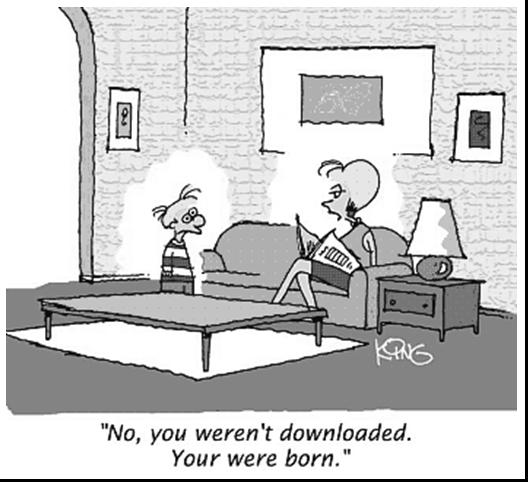
\includegraphics[width=.5\textwidth]{fig1.jpg}
    \caption{Exemplo de como colocar a legenda em uma figura.}
    \label{fig:exemplo}
\end{figure}

A Figura~\ref{fig:exemplo} apresenta um exemplo de como usar e citar uma figura. Sempre comente cada figura no texto.

Aqui temos um exemplo de como citar uma URL na bibliografia~\cite{systemverilog}.

Aqui temos um exemplo de como criar um hiperlink. Veja neste
\href{https://www.youtube.com/watch?v=itWbXy0Qzw0}{link} um exemplo de vídeo publicado. Ao contrário do vídeo deste exemplo, sempre inicie o vídeo apresentando o grupo (nome e semestre), narrando o que é o experimento, os objetivos e descreva o que está sendo feito no vídeo.

Sempre identifique no site do vídeo:
\begin{itemize}
    \item o experimento: Experimento 7;
    \item o semestre: 2022/1;
    \item a disciplina: CIC0231 - Laboratório de Circuitos Lógicos;
    \item a universidade: Universidade de Brasília (UnB);
    \item o grupo: Grupo G37;
    \item os nomes dos componentes do grupo.
\end{itemize}

Desta forma se facilita uma busca pelo vídeo. É apresentado acima como fazer uma listagem não numerada.

\subsection{Demultiplexador}
\label{sec:Demux}

Este é outro item do experimento. Aqui temos um exemplo de como construir e citar uma tabela, conforme mostrado na Tabela~\ref{tab:resultados}.

\begin{table}[H]
    \centering
    \caption{Exemplo de como construir uma tabela.}
    \label{tab:resultados}
    \begin{tabular}{|c|c|c|c|c|c|c|c|}
    \cline{2-7}
    \multicolumn{1}{c}{} & \multicolumn{3}{|c|}{Fase 1} & \multicolumn{3}{c|}{Fase 2} & \multicolumn{1}{c}{} \\
    \hline
    Experimento & $n_g$ & $n_l$ & $n_t$ & $n_g$ & $n_l$ & $n_t$ & $t(s)$ \\
    \hline
    1 bit full adder & 8.16 & 3.8 & 47.6 & 5.03 & 3.0 & 25.93 & 99.13 \\
    2 bits full adder & 18.06 & 5.16 & 107.13 & 11.06 & 4.9 & 60.06 & 709.56 \\
    2 bits multiplier & 14.2 & 4.03 & 74.33 & 7.7 & 2.2 & 37.53 & 357.76 \\
    7 segment decoder & 47.53 & 5.83 & 270.46 & 32.86 & 5.0 & 176.4 & 740.63 \\
    Karnaugh 1 bit full adder & 19.0 & 6.0 & 102.0 & 5.03 & 3.0 & 24.8 & 130.73 \\
    \hline
    \end{tabular}

\end{table}

Aqui devemos colocar uma apresentação e análise da tabela, explicando ao leitor o que se pretende mostrar. A Tabela~\ref{tab:resultados} mostra os tempos de propagação dos diferentes circuitos testados.

As equações devem fazer parte do texto, como 

\begin{equation}
\label{eq:logica}
    Y=AB+\bar{B}\bar{A}
\end{equation}

\noindent onde $A$ e $B$ são as variáveis de entrada. $Y$ a variável de saída. Podemos citar como Equação~\ref{eq:logica}.

Em cada item, após a apresentação dos resultados obtidos, sempre faça uma análise crítica desses resultados.

Dica: Use pesquisa na Internet para tirar as dúvidas sobre edição em \LaTeX .

\section{Conclusões}
\label{sec:Conclusao}

Concluir o relatório explanando rapidamente o que foi feito e os resultados obtidos, sempre correlacionando com os objetivos do experimento apresentados na Seção~\ref{sec:Objetivos}. 


\bibliographystyle{sbc}
\bibliography{relatorio}  %Aqui é a definição do arquivo .bib a ser usado pelas referências


\newpage 
% Colocar aqui apenas as respostas dos itens da Auto-Avaliação
\section*{Auto-Avaliação}

\begin{enumerate}
    \item a
    \item c
    \item b
    \item d
\end{enumerate}


\end{document}
